\documentclass[10pt,a4paper,twocolumn]{article}
\usepackage[utf8]{inputenc}
\raggedbottom
\newcommand{\myvec}[1]{\ensuremath{\begin{pmatrix}#1\end{pmatrix}}}
\usepackage[english]{babel}
\usepackage{amsmath}
%\usepackage{cleveref} 
\usepackage{amsfonts}
\usepackage{amssymb}
\usepackage{graphicx}
\usepackage{multicol}
\setlength{\columnsep}{1cm}
\usepackage[left=2cm,right=2cm,top=2cm,bottom=2cm]{geometry}
\author{N Praful Raj}
\title{\textbf{Assignment-1}}
\numberwithin{equation}{section}
\graphicspath{ {./images/} }
\begin{document}
\maketitle
%\begin {multicols}{1}



	
\section{Problem}
Find the coordinates of the point where the line through$ \myvec{3 \\-4 \\-5}$ and $\myvec{2 \\-3 \\1}$ crosses the plane \begin{align}\myvec{2 & 1 & 1}x=7 \end{align}

\section{Explanation}\label{Explanation}
We know that vector equation of line passing through two points , say A and B is
\begin{align}
\textbf{x} = \vec{A}+\lambda\myvec{\vec{B}-\vec{A}}\label{eq:lineeqn}
\end{align}

We also know that equation of a plane is 
\begin{align}
\textbf{n}^T\textbf{x}=c\label{eq:plane}
\end{align}
Substituting \ref{eq:lineeqn} in \ref{eq:plane} as line passes through the plane we can get the point of contact.

\section{Solution}
\textbf{Step 1}\\
Let us first findout the equation of line passing through two given points using \ref{eq:lineeqn} \\
\\
\begin{align}
\textbf{x}=\myvec{3 \\-4 \\-5}+\lambda 
\myvec{2-3 \\-3+4 \\1+5}
\end{align}
\\

\begin{align}
% \vec{r}=(-\lambda +3)\hat{i}+(\lambda - 4)\hat{j}+(6 \lambda - 5)\hat{k}
\textbf{x}=\myvec{3 \\-4 \\-5}+\lambda 
\myvec{-1 \\1 \\6}\label{eq:lineval}
\end{align}

\textbf{Step 2}\\
Now let us construct the equation of plane from the given data.\\
Using the values we can construct 

\begin{align}
%\hat{n}= \dfrac{2\hat{i}+\hat{j}+\hat{k}}{\sqrt{6}}
\textbf{n}=\myvec{ 2\\ 1\\1}\label{eq:normal}
\end{align}\\
%\begin{align}\label{d}d=\dfrac{|7|}{\sqrt{6}}\end{align}

\textbf{Step 3}\\
Now using \ref{eq:lineval} , \ref{eq:normal}   in \ref{eq:plane}\\

\begin{align}
%\bigg( (-\lambda +3)\hat{i}+(\lambda - 4)\hat{j}+(6 \lambda - 5)\hat{k} \bigg) \cdot \bigg( \dfrac{2\hat{i}+\hat{j}+\hat{k}}{\sqrt{6}} \bigg) = \dfrac{|7|}{\sqrt{6}}
%\textbf{n}^T\textbf{x}=c
\myvec{ 2 && 1 && 1} \Bigg( \myvec{3 \\-4 \\-5}+\lambda\myvec{-1 \\1 \\6} \Bigg)=7\label{eq4}
\end{align}

solving \ref{r1} we get \\
\begin{align}  
6 -4 -5-2\lambda+ \lambda+ 6 \lambda=7 
\end{align}
\\ 
\begin{align} 
5 \lambda=10 
\end{align}

\begin{align}
\lambda=2 \label{eq5} 
\end{align}

Now substituting the value of $\lambda$ in \ref{eq:lineval} we get the point of contact of line on plane

%\begin{align}
%\textbf{x}=\myvec{-2+3\\2-4\\12-5 }
%\end{align}
%\\Therefore the point of contact of line on plane is

\begin{align}
\textbf{x}=\myvec{1\\-2\\7 }
\end{align}
\pagebreak

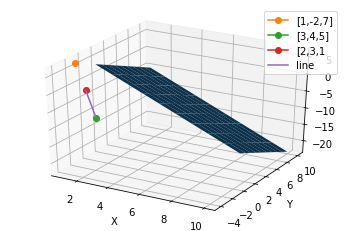
\includegraphics{Figure_3}
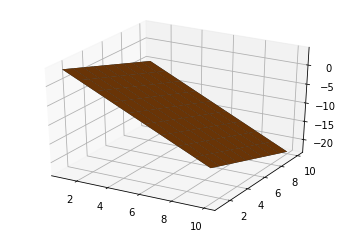
\includegraphics{Figure_4}






%\end{multicols}

\end{document}